\documentclass[12pt,a4paper,oneside]{report}

\usepackage{fontspec}
\setmainfont{TeX Gyre Termes}
\setsansfont{TeX Gyre Heros}
\setmonofont{DejaVu Sans Mono}
\usepackage[vietnamese]{babel}
\usepackage[a4paper,top=2.5cm,bottom=3cm,left=3cm,right=2cm]{geometry}
\usepackage{graphicx}
\usepackage{float}
\usepackage{tabularx}
\usepackage{longtable}
\usepackage{array}
\usepackage{booktabs}
\usepackage{enumitem}
\usepackage[hidelinks]{hyperref}
\usepackage{microtype}
\usepackage{setspace}
\usepackage{caption}
\usepackage{fancyhdr}
\usepackage[fontsize=13pt]{scrextend}
\usepackage{tikz}
\usepackage{xcolor}
\usepackage{indentfirst}
\usepackage{titlesec}
\usepackage{listings}
\usepackage{pdflscape}

\graphicspath{{images/}{diagrams/}}
\setlength{\parindent}{1cm}
\setlength{\parskip}{6pt}
\setstretch{1.3}
\renewcommand{\arraystretch}{1.25}
\setlist[itemize]{leftmargin=1.4cm,itemsep=2pt,topsep=4pt,parsep=0pt}
\setlist[enumerate]{leftmargin=1.4cm,itemsep=2pt,topsep=4pt,parsep=0pt}
\captionsetup{font=normalsize,labelfont=bf}
\pagestyle{fancy}
\fancyhf{}
\fancyfoot[C]{\thepage}
\renewcommand{\headrulewidth}{0pt}
\setcounter{secnumdepth}{3}
\setcounter{tocdepth}{3}
\titleformat{\chapter}[block]
  {\centering\bfseries\fontsize{16pt}{20pt}\selectfont}
  {}{0pt}{}
\titlespacing*{\chapter}{0pt}{0pt}{18pt}
\titleformat{\section}[block]
  {\bfseries\fontsize{14pt}{18pt}\selectfont}
  {\thesection}{0.8em}{}
\titlespacing*{\section}{0pt}{16pt}{6pt}
\titleformat{\subsection}[block]
  {\bfseries\fontsize{13pt}{17pt}\selectfont}
  {\thesubsection}{0.8em}{}
\titlespacing*{\subsection}{0pt}{12pt}{4pt}

\lstset{
  basicstyle=\ttfamily\small,
  breaklines=true,
  frame=single,
  columns=fullflexible,
  keepspaces=true
}

\newcommand{\projectname}{WEB3demo}
\newcommand{\reporttitle}{HỆ THỐNG CHIA SẺ TÀI LIỆU BẢO MẬT DỰA TRÊN VÍ BLOCKCHAIN VÀ PHÊ DUYỆT NHIỀU NGƯỜI}

\hypersetup{
  pdftitle={Báo cáo môn Kỹ thuật phần mềm - WEB3demo},
  pdfauthor={Nhóm 11}
}

\begin{document}
\hypersetup{pageanchor=false}
\pagenumbering{gobble}
\begin{titlepage}
\thispagestyle{empty}
\begin{tikzpicture}[remember picture,overlay]
\draw[line width=1.5pt]
  ([xshift=1.5cm,yshift=-1.5cm]current page.north west)
  rectangle
  ([xshift=-1.5cm,yshift=1.5cm]current page.south east);
\draw[line width=0.5pt]
  ([xshift=1.7cm,yshift=-1.7cm]current page.north west)
  rectangle
  ([xshift=-1.7cm,yshift=1.7cm]current page.south east);
\end{tikzpicture}

\begin{center}
{\fontsize{12pt}{15pt}\selectfont\bfseries
TRƯỜNG ĐẠI HỌC PHENIKAA\\[2pt]
TRƯỜNG CÔNG NGHỆ THÔNG TIN}

\vspace{0.55cm}

\includegraphics[width=4.2cm]{logo.jpg}
\vspace{0.65cm}

{\fontsize{17pt}{22pt}\selectfont\bfseries BÁO CÁO MÔN HỌC}

\vspace{0.25cm}
{\fontsize{14pt}{18pt}\selectfont\bfseries KỸ THUẬT PHẦN MỀM}

\vspace{0.75cm}
{\fontsize{12.5pt}{16pt}\selectfont\itshape Đề tài:}

\vspace{0.35cm}
{\fontsize{14.5pt}{20pt}\selectfont\bfseries
\reporttitle}

\vspace{0.75cm}
\small
\begin{tabular}{@{} p{4.5cm} p{7.1cm} @{}}
  \textbf{Nhóm thực hiện} & Nhóm 11 \\[0.16cm]
  \textbf{Sinh viên} & Hoàng Tiến Đạt -- 23010864 \\
                    & Tô Thị Thùy Dương -- 23010876 \\[0.16cm]
  \textbf{Giảng viên hướng dẫn} & TS. Trịnh Thanh Bình \\
\end{tabular}
\normalsize

\vfill
{\fontsize{12pt}{15pt}\selectfont\bfseries Hà Nội -- 2026}
\end{center}
\end{titlepage}

\begin{titlepage}
\thispagestyle{empty}
\begin{center}
{\fontsize{12pt}{15pt}\selectfont\bfseries
TRƯỜNG ĐẠI HỌC PHENIKAA\\[2pt]
KHOA CÔNG NGHỆ THÔNG TIN}

\vspace{1.8cm}
{\fontsize{16pt}{20pt}\selectfont\bfseries BÁO CÁO MÔN KỸ THUẬT PHẦN MỀM}

\vspace{0.8cm}
{\fontsize{14pt}{20pt}\selectfont\bfseries
\reporttitle}

\vspace{1.5cm}
\begin{tabular}{ll}
\textbf{Tên hệ thống} & : \projectname \\
\textbf{Nhóm thực hiện} & : Nhóm 11 \\
\textbf{Sinh viên} & : Hoàng Tiến Đạt; Tô Thị Thùy Dương \\
\textbf{Công nghệ chính} & : Next.js, React, SQLite, MetaMask, Cloudflare R2 \\
\textbf{Hình thức triển khai} & : Local/Railway, storage local hoặc R2 \\
\end{tabular}

\vfill
{\fontsize{12pt}{15pt}\selectfont Hà Nội -- 2026}
\end{center}
\end{titlepage}

\chapter*{TÓM TẮT}
\addcontentsline{toc}{chapter}{TÓM TẮT}

Báo cáo trình bày quá trình phân tích, thiết kế, cài đặt và kiểm thử hệ thống \projectname{} trong khuôn khổ môn Kỹ thuật phần mềm. Hệ thống giải quyết bài toán chia sẻ tài liệu nhạy cảm sau khi upload: tài liệu được mã hóa phía client, lưu trữ dưới dạng ciphertext, cấp quyền bằng token, hỗ trợ thu hồi quyền và cho phép thiết lập cơ chế phê duyệt nhiều ví đối với tài liệu quan trọng.

Về mặt kỹ thuật, hệ thống sử dụng Next.js và React cho giao diện, Next.js API Routes cho backend, SQLite cho metadata, MetaMask cho định danh người dùng, Web Crypto API cho mã hóa phía trình duyệt và Cloudflare R2 cho lưu trữ ciphertext khi triển khai online. Báo cáo tập trung vào các nội dung của Kỹ thuật phần mềm: khảo sát bài toán, phân tích yêu cầu, thiết kế use case, thiết kế kiến trúc, thiết kế cơ sở dữ liệu, thiết kế API, cài đặt module, kiểm thử và triển khai.

Kết quả đạt được là một prototype có thể demo theo luồng ba ví: A là chủ sở hữu tài liệu, B là người đồng phê duyệt và C là người nhận. C chỉ có thể mở tài liệu khi yêu cầu truy cập đã được A và B phê duyệt đủ ngưỡng. Hệ thống cũng cung cấp dashboard, protected viewer, audit trail, healthcheck và tài liệu triển khai Railway/R2.

\clearpage

\chapter*{LỜI CAM ĐOAN}
\addcontentsline{toc}{chapter}{LỜI CAM ĐOAN}

Nhóm thực hiện cam đoan báo cáo này được xây dựng dựa trên quá trình phân tích và cài đặt hệ thống \projectname{}. Các nội dung tham khảo được ghi nhận trong phần tài liệu tham khảo. Mã nguồn, hình ảnh giao diện và kết quả kiểm thử được lấy từ dự án thực tế trong repository của nhóm.

Nhóm chịu trách nhiệm về tính trung thực của nội dung báo cáo và kết quả trình bày.

\vspace{1cm}
\begin{flushright}
Nhóm thực hiện
\end{flushright}
\clearpage

\chapter*{LỜI CẢM ƠN}
\phantomsection
\addcontentsline{toc}{chapter}{LỜI CẢM ƠN}

Nhóm xin trân trọng cảm ơn TS. Trịnh Thanh Bình, giảng viên hướng dẫn môn Kỹ thuật phần mềm, đã định hướng và góp ý cho nhóm trong quá trình thực hiện đề tài. Những kiến thức thầy truyền đạt về phân tích yêu cầu, thiết kế hệ thống, kiểm thử và triển khai là cơ sở quan trọng để nhóm xây dựng \projectname{} như một hệ thống có cấu trúc thay vì một chức năng đơn lẻ.

Trong quá trình thực hiện, nhóm cũng tham khảo các tài liệu kỹ thuật về Next.js, Web Crypto API, MetaMask, SQLite, Cloudflare R2 và Railway để hoàn thiện sản phẩm demo. Nhóm xin chân thành cảm ơn thầy và mong tiếp tục nhận được góp ý để cải thiện đề tài.

\clearpage

\tableofcontents
\clearpage
\phantomsection
\addcontentsline{toc}{chapter}{DANH MỤC HÌNH ẢNH}
\listoffigures
\clearpage
\phantomsection
\addcontentsline{toc}{chapter}{DANH MỤC BẢNG}
\listoftables
\clearpage
\hypersetup{pageanchor=true}
\pagenumbering{arabic}
\setcounter{page}{1}

\chapter*{MỞ ĐẦU}
\addcontentsline{toc}{chapter}{MỞ ĐẦU}

\section*{1. Lý do chọn đề tài}
\addcontentsline{toc}{section}{1. Lý do chọn đề tài}

Trong môi trường học thuật và nghiên cứu, việc chia sẻ tài liệu như bài báo khoa học, luận văn, báo cáo nội bộ hoặc dữ liệu thí nghiệm diễn ra thường xuyên. Tuy nhiên, các hình thức chia sẻ phổ biến như gửi file qua email, tải lên dịch vụ lưu trữ đám mây hoặc gửi link công khai thường khiến chủ sở hữu mất dần quyền kiểm soát sau khi tài liệu đã rời khỏi thiết bị cá nhân. Người nhận có thể tải bản gốc, chuyển tiếp cho người khác hoặc giữ file sau khi quyền truy cập đáng lẽ đã hết hạn.

Vấn đề đặt ra không chỉ là "làm sao gửi được file", mà là "làm sao kiểm soát vòng đời quyền truy cập của tài liệu sau khi gửi". Đây là một bài toán phù hợp với môn Kỹ thuật phần mềm vì cần kết hợp nhiều khía cạnh: phân tích yêu cầu, thiết kế tác nhân, thiết kế cơ sở dữ liệu, thiết kế giao diện, luồng nghiệp vụ, kiểm thử, triển khai và đánh giá rủi ro.

Từ nhu cầu đó, nhóm lựa chọn đề tài \textbf{\projectname{} -- hệ thống chia sẻ tài liệu bảo mật dựa trên ví blockchain và phê duyệt nhiều người}. Hệ thống không hướng tới việc thay thế hoàn toàn các nền tảng lưu trữ lớn, mà tập trung chứng minh một mô hình phần mềm trong đó tài liệu được mã hóa trước khi upload, quyền truy cập được cấp bằng token, và một số tài liệu nhạy cảm cần nhiều ví cùng phê duyệt trước khi người nhận có thể mở.

\section*{2. Mục tiêu đề tài}
\addcontentsline{toc}{section}{2. Mục tiêu đề tài}

Đề tài hướng tới các mục tiêu chính:

\begin{itemize}
  \item Xây dựng một prototype cho phép người dùng đăng nhập bằng ví MetaMask.
  \item Mã hóa tài liệu phía trình duyệt trước khi upload lên storage.
  \item Thiết kế cơ chế cấp, kiểm tra, thu hồi token truy cập.
  \item Hỗ trợ protected viewer để người nhận xem tài liệu theo quyền được cấp.
  \item Xây dựng cơ chế phê duyệt ngưỡng: A và B cùng duyệt thì C mới nhận quyền mở.
  \item Cung cấp dashboard quản lý tài liệu, token, kho nhóm, yêu cầu phê duyệt và audit trail.
  \item Triển khai được theo hai chế độ: local để demo ổn định và Railway/R2 để demo online.
  \item Kiểm thử các luồng chính bằng lint, build và Playwright E2E.
\end{itemize}

\section*{3. Phạm vi đề tài}
\addcontentsline{toc}{section}{3. Phạm vi đề tài}

Trong phạm vi môn học, hệ thống tập trung vào các chức năng cốt lõi của chia sẻ tài liệu bảo mật:

\begin{itemize}
  \item Định danh người dùng bằng ví, không xây dựng hệ thống mật khẩu truyền thống.
  \item Mã hóa file phía client và lưu ciphertext trên local storage hoặc Cloudflare R2.
  \item Quản lý metadata bằng SQLite.
  \item Phân quyền theo token, vai trò trong kho nhóm và yêu cầu phê duyệt.
  \item Triển khai prototype bằng Next.js, Docker và Railway.
\end{itemize}

Đề tài chưa hướng tới các yêu cầu sản xuất quy mô lớn như phân tán database, giám sát production đầy đủ, chống chụp màn hình tuyệt đối hoặc chứng minh zero-knowledge hoàn chỉnh. Những nội dung này được xem là hướng phát triển.

\section*{4. Phương pháp thực hiện}
\addcontentsline{toc}{section}{4. Phương pháp thực hiện}

Nhóm thực hiện đề tài theo quy trình gần với mô hình lặp:

\begin{enumerate}
  \item Khảo sát bài toán chia sẻ tài liệu nhạy cảm và xác định các rủi ro chính.
  \item Phân tích tác nhân, use case, yêu cầu chức năng và phi chức năng.
  \item Thiết kế kiến trúc tổng quan, cơ sở dữ liệu, API và luồng nghiệp vụ.
  \item Cài đặt từng module: xác thực ví, upload, mã hóa, token, approval, viewer, dashboard.
  \item Kiểm thử bằng lint, production build, API test và E2E test.
  \item Triển khai local/Railway, cấu hình Cloudflare R2 và chuẩn bị kịch bản demo.
\end{enumerate}

\section*{5. Bố cục báo cáo}
\addcontentsline{toc}{section}{5. Bố cục báo cáo}

Báo cáo gồm sáu chương:

\begin{itemize}
  \item Chương 1 trình bày tổng quan đề tài và cơ sở lý thuyết.
  \item Chương 2 phân tích yêu cầu phần mềm.
  \item Chương 3 trình bày phân tích và thiết kế hệ thống.
  \item Chương 4 mô tả quá trình cài đặt hệ thống.
  \item Chương 5 trình bày kiểm thử, triển khai và đánh giá.
  \item Chương 6 tổng kết kết quả và hướng phát triển.
\end{itemize}

\clearpage

\chapter*{CHƯƠNG 1: TỔNG QUAN ĐỀ TÀI VÀ CƠ SỞ LÝ THUYẾT}
\addcontentsline{toc}{chapter}{CHƯƠNG 1: TỔNG QUAN ĐỀ TÀI VÀ CƠ SỞ LÝ THUYẾT}

Chương này trình bày bối cảnh bài toán và các khái niệm kỹ thuật làm nền tảng cho hệ thống \projectname{}. Các nội dung gồm chia sẻ tài liệu bảo mật, mã hóa phía client, định danh bằng ví blockchain, token truy cập, phê duyệt nhiều người, audit trail và lưu trữ object storage.

\section*{1.1. Bài toán chia sẻ tài liệu bảo mật}
\addcontentsline{toc}{section}{1.1. Bài toán chia sẻ tài liệu bảo mật}

Chia sẻ tài liệu thông thường thường dựa trên mô hình người gửi tải file lên server, sau đó người nhận tải bản gốc xuống. Mô hình này đơn giản nhưng tạo ra nhiều rủi ro đối với tài liệu nhạy cảm. Khi bản gốc được lưu trên server hoặc đã tải về thiết bị người nhận, chủ sở hữu khó kiểm soát việc sao chép, chuyển tiếp hoặc sử dụng sau thời hạn cho phép.

Trong bối cảnh học thuật, tài liệu như bài báo chưa công bố, luận văn, đề cương nghiên cứu hoặc dữ liệu thí nghiệm có thể cần chia sẻ với người hướng dẫn, đồng tác giả hoặc hội đồng duyệt. Các tài liệu này cần cơ chế kiểm soát chặt hơn so với link tải thông thường: người nhận phải đúng danh tính, quyền truy cập có thời hạn, có thể thu hồi, và một số trường hợp cần nhiều người đồng ý trước khi mở.

\section*{1.2. Mã hóa phía client}
\addcontentsline{toc}{section}{1.2. Mã hóa phía client}

Mã hóa phía client là phương pháp trong đó dữ liệu được mã hóa ngay trên thiết bị người dùng trước khi gửi đến server. Với cách này, server chỉ nhận ciphertext, không trực tiếp nhận plaintext. Trong \projectname{}, hướng tiếp cận này giúp giảm mức độ tin cậy bắt buộc đặt vào server.

Về mặt thiết kế, mã hóa phía client có ba lợi ích chính:

\begin{itemize}
  \item Giảm rủi ro lộ nội dung nếu storage hoặc server bị truy cập trái phép.
  \item Tách rõ vai trò giữa storage ciphertext và metadata phân quyền.
  \item Phù hợp với mục tiêu privacy-by-design trong chia sẻ tài liệu nhạy cảm.
\end{itemize}

Hệ thống sử dụng Web Crypto API của trình duyệt để thực hiện các thao tác mật mã. Đây là API chuẩn, tránh việc tự triển khai thuật toán mật mã bằng JavaScript thủ công.

\section*{1.3. Định danh bằng ví blockchain}
\addcontentsline{toc}{section}{1.3. Định danh bằng ví blockchain}

Thay vì dùng tài khoản mật khẩu, hệ thống sử dụng ví MetaMask để xác thực người dùng. Quy trình cơ bản gồm:

\begin{enumerate}
  \item Server sinh một thông điệp nonce.
  \item Người dùng ký thông điệp bằng ví MetaMask.
  \item Server xác minh chữ ký để biết người dùng sở hữu địa chỉ ví đó.
  \item Nếu hợp lệ, server tạo session bằng JWT cookie.
\end{enumerate}

Cách làm này giúp hệ thống không cần lưu mật khẩu. Địa chỉ ví trở thành định danh chính trong các bảng như tài liệu, token, thành viên kho, yêu cầu phê duyệt và audit event.

\section*{1.4. Token truy cập và vòng đời quyền}
\addcontentsline{toc}{section}{1.4. Token truy cập và vòng đời quyền}

Token truy cập là mã đại diện cho quyền mở một tài liệu trong một phạm vi nhất định. Trong hệ thống, token có thể gắn với file, người nhận, thời hạn, trạng thái thu hồi và mục đích sử dụng. Token giúp tách quyền truy cập khỏi bản thân file: file vẫn tồn tại ở dạng ciphertext, còn việc người dùng có được lấy ciphertext và giải mã hay không phụ thuộc vào token và chính sách.

Vòng đời token gồm:

\begin{itemize}
  \item Được tạo khi chủ sở hữu chia sẻ tài liệu hoặc khi yêu cầu phê duyệt đủ ngưỡng.
  \item Được kiểm tra trước khi người nhận mở tài liệu.
  \item Có thể hết hạn theo thời gian.
  \item Có thể bị chủ sở hữu thu hồi.
  \item Bị vô hiệu khi tài liệu bị hủy.
\end{itemize}

\section*{1.5. Phê duyệt nhiều người}
\addcontentsline{toc}{section}{1.5. Phê duyệt nhiều người}

Phê duyệt nhiều người là cơ chế yêu cầu nhiều thành viên cùng xác nhận trước khi cấp quyền truy cập. Trong \projectname{}, kịch bản trọng tâm là A và B cùng duyệt thì C mới nhận token mở tài liệu. Cơ chế này phù hợp với tài liệu quan trọng cần kiểm soát chặt, chẳng hạn tài liệu nghiên cứu chưa công bố hoặc hồ sơ nội bộ.

Về mặt phần mềm, phê duyệt nhiều người gồm các thành phần:

\begin{itemize}
  \item Chính sách ngưỡng trong kho nhóm.
  \item Các share được mã hóa cho từng thành viên.
  \item Yêu cầu truy cập do người nhận tạo.
  \item Đóng góp phê duyệt của từng người duyệt.
  \item Token chỉ được phát hành khi số phê duyệt đạt ngưỡng.
\end{itemize}

\section*{1.6. Audit trail}
\addcontentsline{toc}{section}{1.6. Audit trail}

Audit trail là nhật ký ghi lại các hành động quan trọng trong hệ thống, ví dụ tạo file, tạo token, thu hồi token, duyệt yêu cầu hoặc hủy tài liệu. Audit trail không ngăn chặn rủi ro trực tiếp, nhưng giúp truy vết và giải thích vòng đời truy cập.

Trong dự án, bảng \code{audit\_events} được thiết kế với trigger ngăn cập nhật và xóa. Điều này giúp minh họa nguyên tắc nhật ký bất biến ở mức prototype.

\section*{1.7. Cloud object storage}
\addcontentsline{toc}{section}{1.7. Cloud object storage}

Cloudflare R2 được dùng như object storage để lưu ciphertext khi triển khai online. Hệ thống không lưu bản gốc lên R2; mỗi object là dữ liệu đã mã hóa. Metadata như tên file, mime type, owner, token, approval và audit được lưu ở SQLite.

Cách tách này có lợi cho thiết kế hệ thống:

\begin{itemize}
  \item Storage chỉ cần lưu object theo khóa nội dung.
  \item Backend có thể đổi provider storage mà không thay đổi logic nghiệp vụ chính.
  \item Khi chạy local, hệ thống vẫn có thể dùng local filesystem để demo nhanh.
\end{itemize}

\clearpage

\chapter*{CHƯƠNG 2: KHẢO SÁT VÀ PHÂN TÍCH YÊU CẦU}
\phantomsection
\addcontentsline{toc}{chapter}{CHƯƠNG 2: KHẢO SÁT VÀ PHÂN TÍCH YÊU CẦU}

Chương này phân tích yêu cầu hệ thống theo góc nhìn Kỹ thuật phần mềm. Nội dung gồm tác nhân, use case, yêu cầu chức năng, yêu cầu phi chức năng, ràng buộc và giả định.

\section*{2.1. Tác nhân hệ thống}
\phantomsection
\addcontentsline{toc}{section}{2.1. Tác nhân hệ thống}

\begin{table}[H]
\centering
\caption{Các tác nhân chính của hệ thống}
\begin{tabularx}{\textwidth}{|p{3.2cm}|X|}
\hline
\textbf{Tác nhân} & \textbf{Mô tả} \\ \hline
Chủ sở hữu tài liệu & Người upload, mã hóa, chia sẻ, thu hồi token và hủy tài liệu. Trong demo là ví A. \\ \hline
Người phê duyệt & Thành viên có quyền tham gia duyệt yêu cầu mở tài liệu nhạy cảm. Trong demo là ví B. \\ \hline
Người nhận & Người được cấp token hoặc tạo yêu cầu truy cập để mở tài liệu. Trong demo là ví C. \\ \hline
Thành viên kho & Người thuộc một kho nhóm với vai trò owner, editor hoặc viewer. \\ \hline
Cloudflare R2 & Dịch vụ lưu trữ object, chỉ nhận ciphertext. \\ \hline
\end{tabularx}
\end{table}

\section*{2.2. Use case tổng quát}
\phantomsection
\addcontentsline{toc}{section}{2.2. Use case tổng quát}

Hình \ref{fig:usecase} thể hiện use case tổng quát của hệ thống. Sơ đồ được viết bằng PlantUML để dễ bảo trì và tái sinh khi thay đổi yêu cầu.

\begin{figure}[H]
\centering
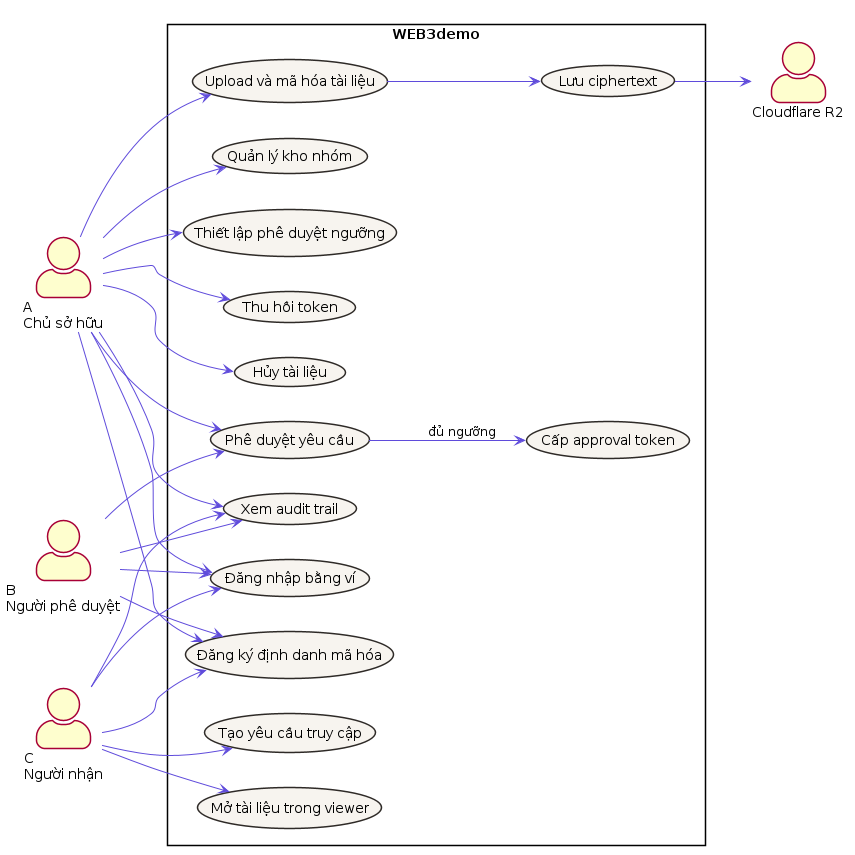
\includegraphics[width=\textwidth]{usecase.png}
\caption{Sơ đồ use case tổng quát của WEB3demo}
\label{fig:usecase}
\end{figure}

\section*{2.3. Yêu cầu chức năng}
\phantomsection
\addcontentsline{toc}{section}{2.3. Yêu cầu chức năng}

\begin{longtable}{|p{2cm}|p{5cm}|p{7cm}|}
\caption{Danh sách yêu cầu chức năng} \\
\hline
\textbf{Mã} & \textbf{Yêu cầu} & \textbf{Mô tả} \\ \hline
FR-01 & Đăng nhập bằng ví & Người dùng ký nonce bằng MetaMask để tạo session. \\ \hline
FR-02 & Đăng ký định danh mã hóa & Người dùng đăng ký public key để nhận key envelope hoặc share mã hóa. \\ \hline
FR-03 & Upload tài liệu & Chủ sở hữu chọn file, hệ thống mã hóa phía client và upload ciphertext. \\ \hline
FR-04 & Tạo metadata file & Backend lưu cid, tên file, mime, owner, iv, access mode và thông tin khóa. \\ \hline
FR-05 & Tạo token chia sẻ & Chủ sở hữu tạo token có thời hạn cho tài liệu. \\ \hline
FR-06 & Kiểm tra token & Người nhận nhập token, hệ thống kiểm tra hết hạn, thu hồi và quyền ví. \\ \hline
FR-07 & Thu hồi token & Chủ sở hữu có thể vô hiệu hóa token đã cấp. \\ \hline
FR-08 & Hủy tài liệu & Chủ sở hữu hủy tài liệu, thu hồi token và dọn ciphertext nếu phù hợp. \\ \hline
FR-09 & Quản lý kho nhóm & Người dùng tạo kho, thêm thành viên và gán vai trò. \\ \hline
FR-10 & Thiết lập phê duyệt ngưỡng & Kho nhóm có thể bật chính sách K-of-N. \\ \hline
FR-11 & Tạo yêu cầu truy cập & Người nhận tạo yêu cầu mở tài liệu cần phê duyệt. \\ \hline
FR-12 & Phê duyệt yêu cầu & Thành viên hợp lệ gửi contribution cho yêu cầu truy cập. \\ \hline
FR-13 & Cấp approval token & Khi đủ ngưỡng, hệ thống tạo token cho người yêu cầu. \\ \hline
FR-14 & Protected viewer & Người nhận mở tài liệu trong viewer thay vì tải bản gốc theo mặc định. \\ \hline
FR-15 & Audit trail & Hệ thống ghi lại các hành động quan trọng. \\ \hline
\end{longtable}

\section*{2.4. Yêu cầu phi chức năng}
\phantomsection
\addcontentsline{toc}{section}{2.4. Yêu cầu phi chức năng}

\begin{table}[H]
\centering
\caption{Yêu cầu phi chức năng}
\begin{tabularx}{\textwidth}{|p{3.5cm}|X|}
\hline
\textbf{Nhóm yêu cầu} & \textbf{Cách đáp ứng trong hệ thống} \\ \hline
Bảo mật & Mã hóa phía client, JWT cookie, CSRF protection, token thu hồi, kiểm tra vai trò và audit log. \\ \hline
Riêng tư & Server không chủ động lưu plaintext; storage chỉ lưu ciphertext. \\ \hline
Khả dụng & Có thể chạy local nếu deploy online gặp sự cố; có healthcheck kiểm tra runtime. \\ \hline
Bảo trì & Tách module theo API, component, storage helper, db helper, audit helper và access-control helper. \\ \hline
Mở rộng & Storage có abstraction để dùng local hoặc Cloudflare R2; kiến trúc có thể phát triển sang IPFS/Filecoin. \\ \hline
Kiểm thử & Có ESLint, Next build và Playwright E2E cho các luồng quan trọng. \\ \hline
\end{tabularx}
\end{table}

\section*{2.5. Ràng buộc và giả định}
\phantomsection
\addcontentsline{toc}{section}{2.5. Ràng buộc và giả định}

Các ràng buộc chính:

\begin{itemize}
  \item Người dùng cần trình duyệt hỗ trợ Web Crypto API và MetaMask.
  \item SQLite phù hợp prototype và demo một instance; nếu scale lớn cần chuyển sang PostgreSQL hoặc database managed.
  \item Protected viewer không thể ngăn tuyệt đối việc người dùng chụp màn hình bằng thiết bị khác.
  \item R2 key phải được bảo vệ và không được commit vào repository.
  \item Khi deploy Railway, thư mục chứa SQLite cần được mount bằng volume.
\end{itemize}

\clearpage

\chapter*{CHƯƠNG 3: PHÂN TÍCH VÀ THIẾT KẾ HỆ THỐNG}
\phantomsection
\addcontentsline{toc}{chapter}{CHƯƠNG 3: PHÂN TÍCH VÀ THIẾT KẾ HỆ THỐNG}

Chương này trình bày thiết kế hệ thống \projectname{} ở mức kiến trúc, dữ liệu, API và luồng xử lý. Mục tiêu của chương là cho thấy hệ thống được thiết kế như một phần mềm có cấu trúc, không phải chỉ là một trang web upload file đơn giản.

\section*{3.1. Kiến trúc tổng quan}
\phantomsection
\addcontentsline{toc}{section}{3.1. Kiến trúc tổng quan}

Hệ thống được chia thành ba vùng chính: trình duyệt người dùng, ứng dụng Next.js và tầng lưu trữ. Trình duyệt chịu trách nhiệm tương tác ví và mã hóa/giải mã. Backend chịu trách nhiệm xác thực, phân quyền, quản lý metadata và audit. Storage chỉ lưu ciphertext.

\begin{figure}[H]
\centering
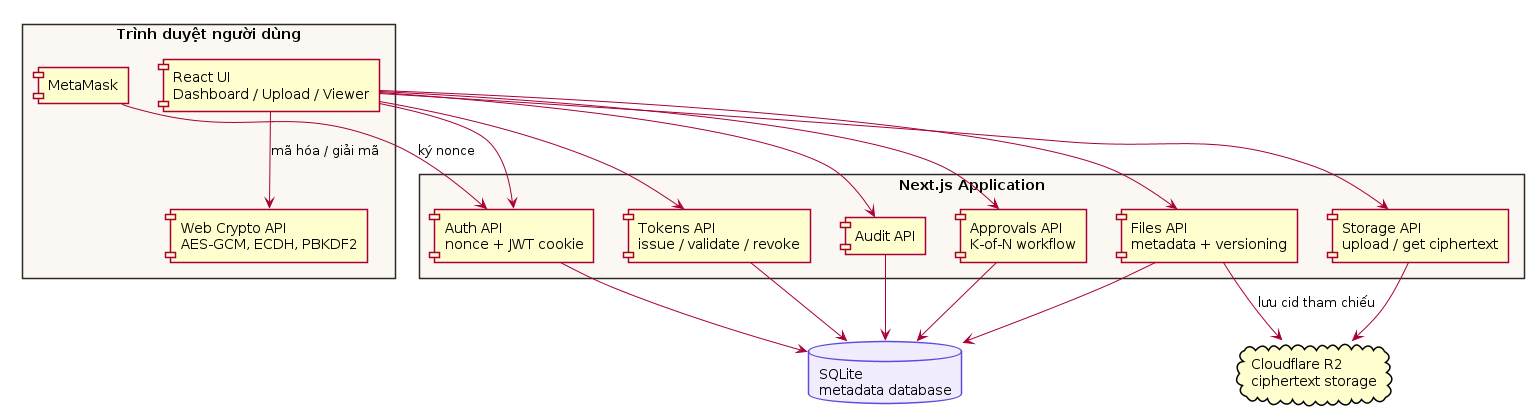
\includegraphics[width=\textwidth]{architecture.png}
\caption{Kiến trúc tổng quan của hệ thống}
\label{fig:architecture}
\end{figure}

Cách phân tách này có các ưu điểm:

\begin{itemize}
  \item Logic nhạy cảm về nội dung file nằm ở client.
  \item Backend tập trung vào quyền truy cập và vòng đời tài liệu.
  \item Storage có thể thay thế giữa local filesystem và Cloudflare R2.
  \item Dễ kiểm thử từng tầng: UI, API, database và storage.
\end{itemize}

\section*{3.2. Thiết kế module}
\phantomsection
\addcontentsline{toc}{section}{3.2. Thiết kế module}

\begin{table}[H]
\centering
\caption{Các module chính trong hệ thống}
\begin{tabularx}{\textwidth}{|p{3.5cm}|X|}
\hline
\textbf{Module} & \textbf{Trách nhiệm} \\ \hline
Auth module & Tạo nonce, xác minh chữ ký ví, tạo JWT session và đăng xuất. \\ \hline
Encryption identity module & Lưu public key của ví để phục vụ key envelope và threshold share. \\ \hline
File module & Lưu metadata file, version, access mode, vault và trạng thái hủy. \\ \hline
Storage module & Upload, lấy, kiểm tra và xóa ciphertext từ local hoặc R2. \\ \hline
Token module & Cấp, kiểm tra, liệt kê và thu hồi token truy cập. \\ \hline
Vault module & Quản lý kho nhóm, thành viên và vai trò. \\ \hline
Approval module & Quản lý yêu cầu phê duyệt, contribution và approval token. \\ \hline
Audit module & Ghi và truy vấn các sự kiện quan trọng. \\ \hline
UI module & Dashboard, upload wizard, downloader, viewer và thông báo. \\ \hline
\end{tabularx}
\end{table}

\section*{3.3. Thiết kế cơ sở dữ liệu}
\phantomsection
\addcontentsline{toc}{section}{3.3. Thiết kế cơ sở dữ liệu}

Hệ thống sử dụng SQLite cho metadata. Dữ liệu file thực tế không lưu trong database mà lưu ở storage dưới dạng ciphertext, còn database lưu cid và thông tin quyền.

\small
\begin{longtable}{|p{4.6cm}|p{8.5cm}|}
\caption{Các bảng dữ liệu chính} \\
\hline
\textbf{Bảng} & \textbf{Vai trò} \\ \hline
\seqsplit{files} & Lưu metadata tài liệu: owner, cid, tên file, mime, kích thước, iv, access mode, version, vault, trạng thái hủy. \\ \hline
\seqsplit{tokens} & Lưu token truy cập, file tương ứng, người nhận, thời hạn, trạng thái thu hồi và mục đích token. \\ \hline
\seqsplit{encryption\_identities} & Lưu public key của ví và chữ ký xác nhận public key thuộc về ví đó. \\ \hline
\seqsplit{key\_envelopes} & Lưu key envelope cho token đích danh. \\ \hline
\seqsplit{vaults} & Lưu thông tin kho nhóm. \\ \hline
\seqsplit{vault\_members} & Lưu thành viên kho và vai trò owner/editor/viewer. \\ \hline
\seqsplit{vault\_threshold\_policies} & Lưu chính sách phê duyệt ngưỡng của kho. \\ \hline
\seqsplit{threshold\_file\_shares} & Lưu các share đã mã hóa cho từng thành viên. \\ \hline
\seqsplit{approval\_requests} & Lưu yêu cầu truy cập của người nhận. \\ \hline
\seqsplit{approval\_contributions} & Lưu đóng góp phê duyệt của từng người duyệt. \\ \hline
\seqsplit{audit\_events} & Lưu nhật ký hành động quan trọng; có trigger ngăn sửa/xóa. \\ \hline
\seqsplit{rate\_limits} & Lưu bộ đếm giới hạn request cho API nhạy cảm. \\ \hline
\end{longtable}
\normalsize

Một số quan hệ quan trọng:

\begin{itemize}
  \item Một file có thể có nhiều token.
  \item Một vault có nhiều thành viên và một chính sách phê duyệt.
  \item Một yêu cầu phê duyệt thuộc về một file và một requester.
  \item Một yêu cầu có nhiều contribution từ các người duyệt khác nhau.
  \item Audit event gắn với actor, action, resource type và resource id.
\end{itemize}

\section*{3.4. Thiết kế API}
\phantomsection
\addcontentsline{toc}{section}{3.4. Thiết kế API}

\small
\begin{longtable}{|p{1.8cm}|p{4.5cm}|p{6.8cm}|}
\caption{Nhóm API chính} \\
\hline
\textbf{Phương thức} & \textbf{Endpoint} & \textbf{Mục đích} \\ \hline
POST & \seqsplit{/api/auth/start} & Sinh thông điệp nonce để ví ký. \\ \hline
POST & \seqsplit{/api/auth/verify} & Xác minh chữ ký ví và tạo session. \\ \hline
POST & \seqsplit{/api/storage/upload} & Nhận ciphertext và lưu vào provider storage. \\ \hline
GET & \seqsplit{/api/storage/get} & Trả ciphertext nếu token hoặc approval hợp lệ. \\ \hline
POST & \seqsplit{/api/files} & Tạo metadata file, token và share nếu có. \\ \hline
DELETE & \seqsplit{/api/files/[id]} & Chủ sở hữu hủy tài liệu. \\ \hline
POST & \seqsplit{/api/tokens/issue} & Cấp token mới cho file. \\ \hline
POST & \seqsplit{/api/tokens/validate} & Kiểm tra token trước khi mở file. \\ \hline
POST & \seqsplit{/api/tokens/revoke} & Thu hồi token. \\ \hline
GET & \seqsplit{/api/approvals} & Liệt kê yêu cầu phê duyệt liên quan đến người dùng. \\ \hline
POST & \seqsplit{/api/approvals/[id]/approve} & Gửi contribution phê duyệt cho yêu cầu. \\ \hline
GET & \seqsplit{/api/audit} & Truy vấn audit event được phép xem. \\ \hline
GET & \seqsplit{/api/health} & Kiểm tra database và provider storage. \\ \hline
\end{longtable}
\normalsize

\section*{3.5. Thiết kế luồng upload và chia sẻ}
\phantomsection
\addcontentsline{toc}{section}{3.5. Thiết kế luồng upload và chia sẻ}

Luồng upload gồm các bước:

\begin{enumerate}
  \item Người dùng kết nối ví và có session hợp lệ.
  \item Người dùng chọn file trong upload wizard.
  \item Trình duyệt tạo khóa mã hóa và mã hóa file bằng Web Crypto.
  \item Client upload ciphertext lên \code{/api/storage/upload}.
  \item Storage trả về \code{cid}.
  \item Client gửi metadata, iv, access mode và key material hợp lệ tới \code{/api/files}.
  \item Backend lưu metadata, tạo token ban đầu và ghi audit event.
\end{enumerate}

Điểm quan trọng là file rõ chỉ tồn tại tại trình duyệt. Backend không nhận file gốc trong thiết kế chủ đích.

\section*{3.6. Thiết kế luồng phê duyệt A+B cho C}
\phantomsection
\addcontentsline{toc}{section}{3.6. Thiết kế luồng phê duyệt A+B cho C}

Luồng phê duyệt được thiết kế để minh họa kiểm soát truy cập nhiều người. Hình \ref{fig:approvalseq} mô tả trình tự chính.

\begin{figure}[H]
\centering
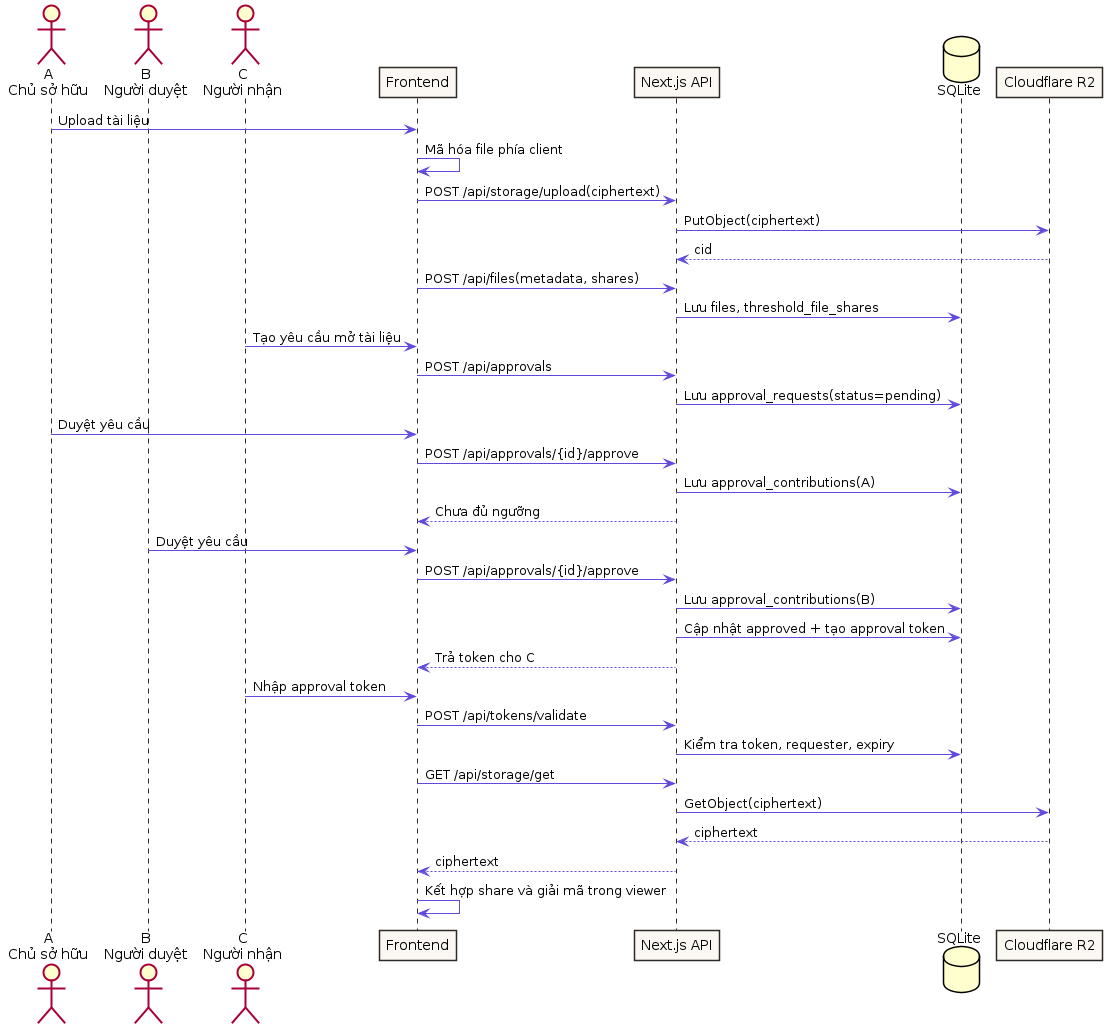
\includegraphics[width=\textwidth]{approval-sequence.png}
\caption{Sequence diagram luồng phê duyệt A+B cho C}
\label{fig:approvalseq}
\end{figure}

Các quy tắc chính:

\begin{itemize}
  \item Người yêu cầu không được tự phê duyệt yêu cầu của mình.
  \item Contribution của mỗi người duyệt chỉ được tính một lần.
  \item Token approval chỉ được tạo khi số contribution hợp lệ đạt ngưỡng.
  \item Token approval gắn với requester, không phải token mở tự do cho mọi ví.
\end{itemize}

\section*{3.7. Thiết kế giao diện}
\phantomsection
\addcontentsline{toc}{section}{3.7. Thiết kế giao diện}

Giao diện gồm bốn màn hình chính: giới thiệu, upload, dashboard và viewer. Các màn hình dùng chung hệ nhận diện, chuyển động và logo của dự án.

\clearpage
\begin{figure}[H]
\centering
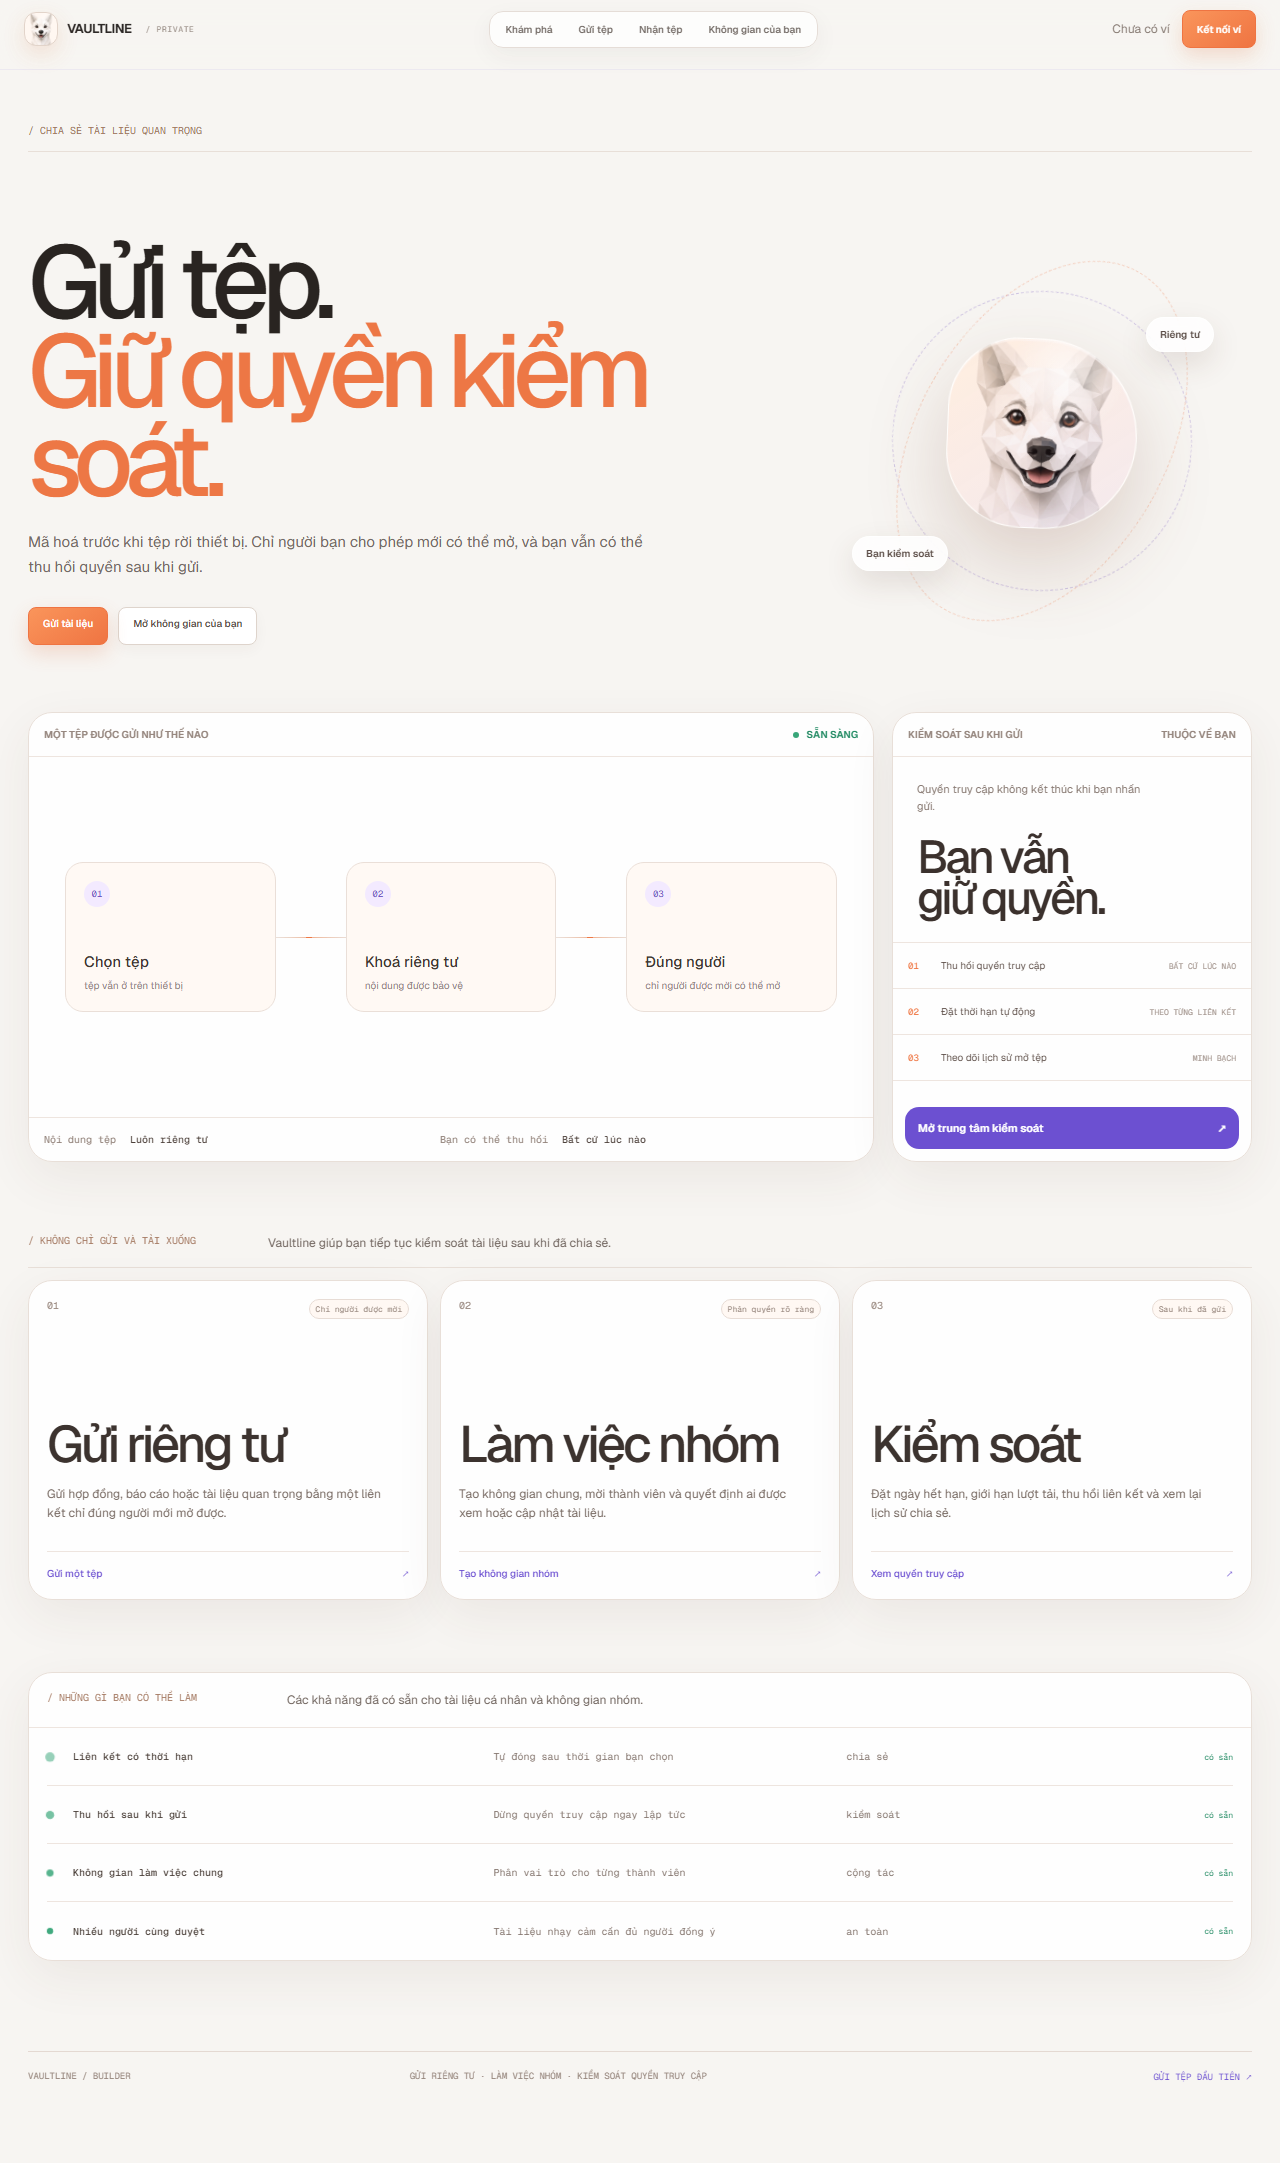
\includegraphics[width=\textwidth,height=0.74\textheight,keepaspectratio]{live-home.png}
\caption{Trang giới thiệu hệ thống}
\end{figure}

\begin{figure}[H]
\centering
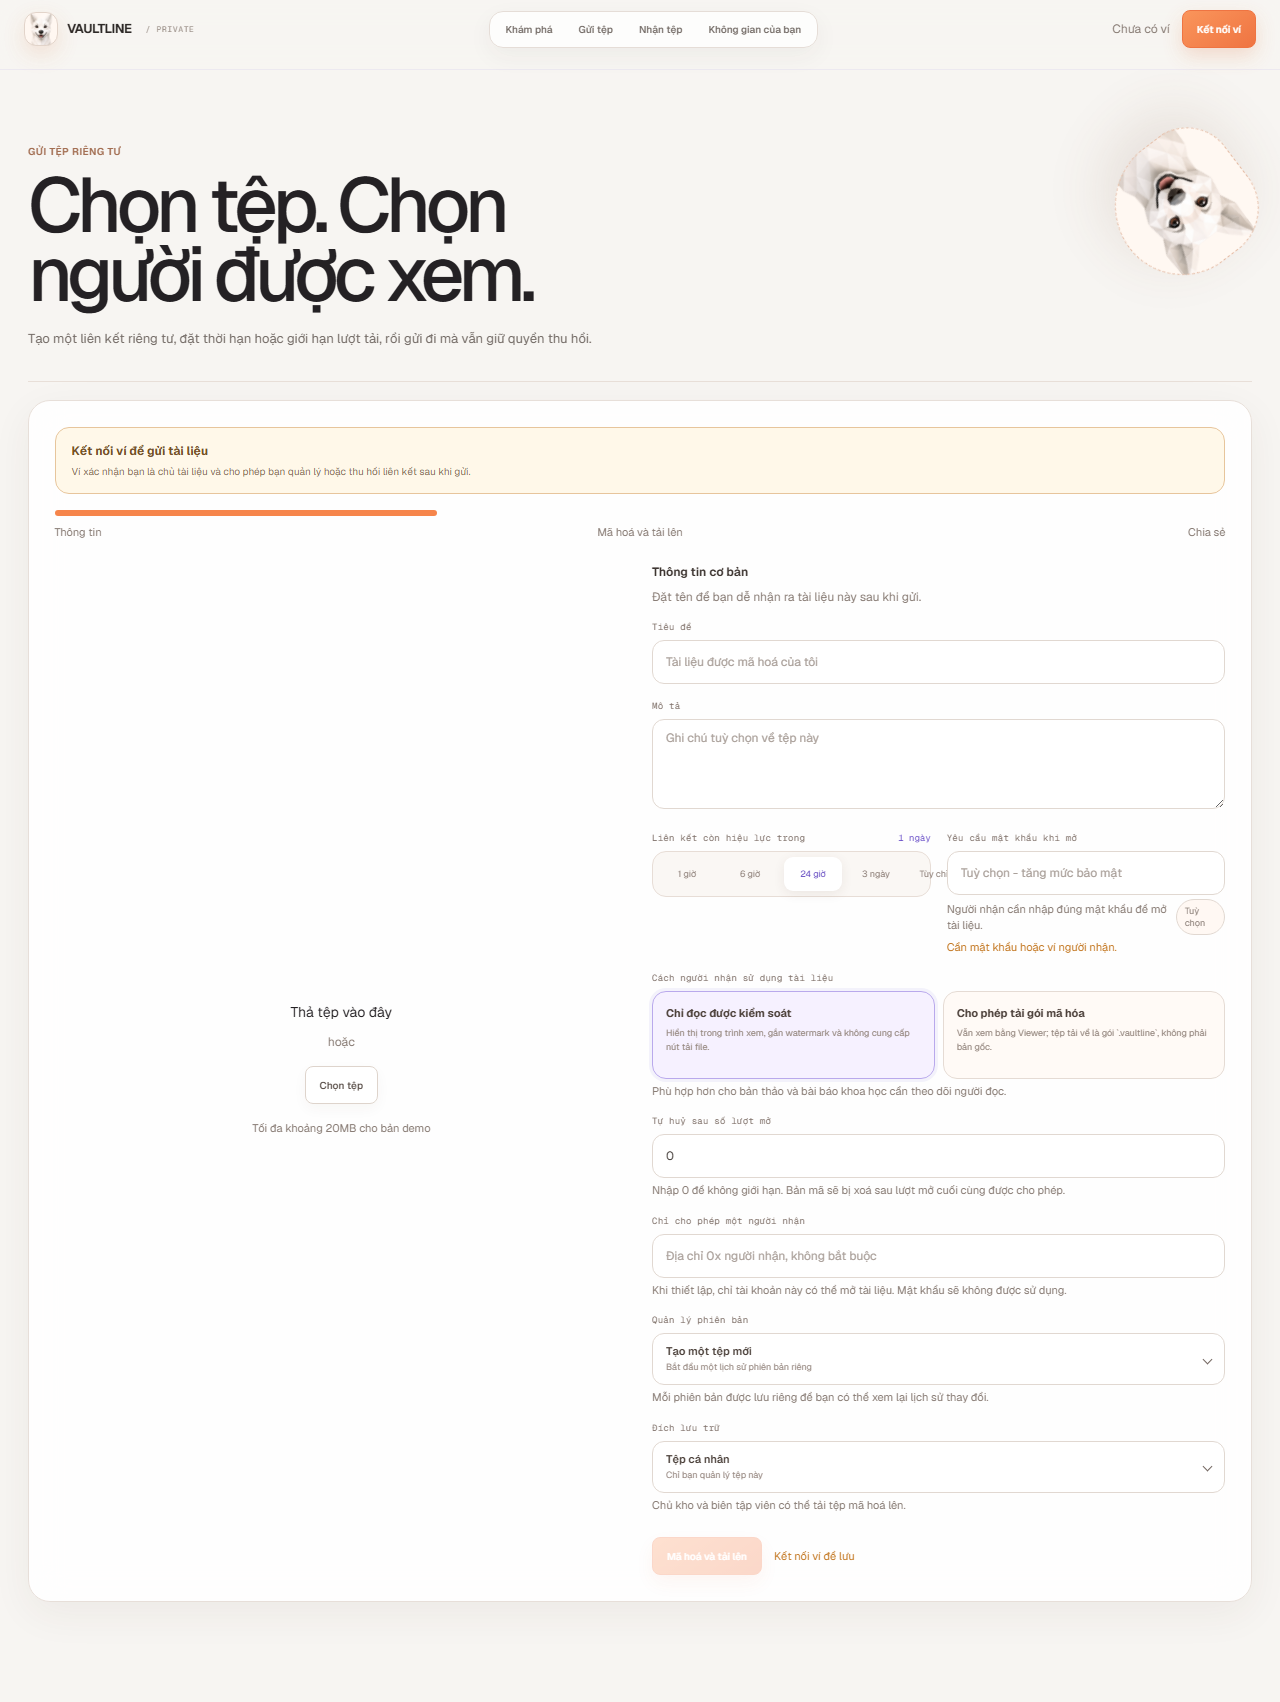
\includegraphics[width=\textwidth,height=0.74\textheight,keepaspectratio]{live-upload.png}
\caption{Upload wizard và thiết lập quyền chia sẻ}
\end{figure}

\begin{figure}[H]
\centering
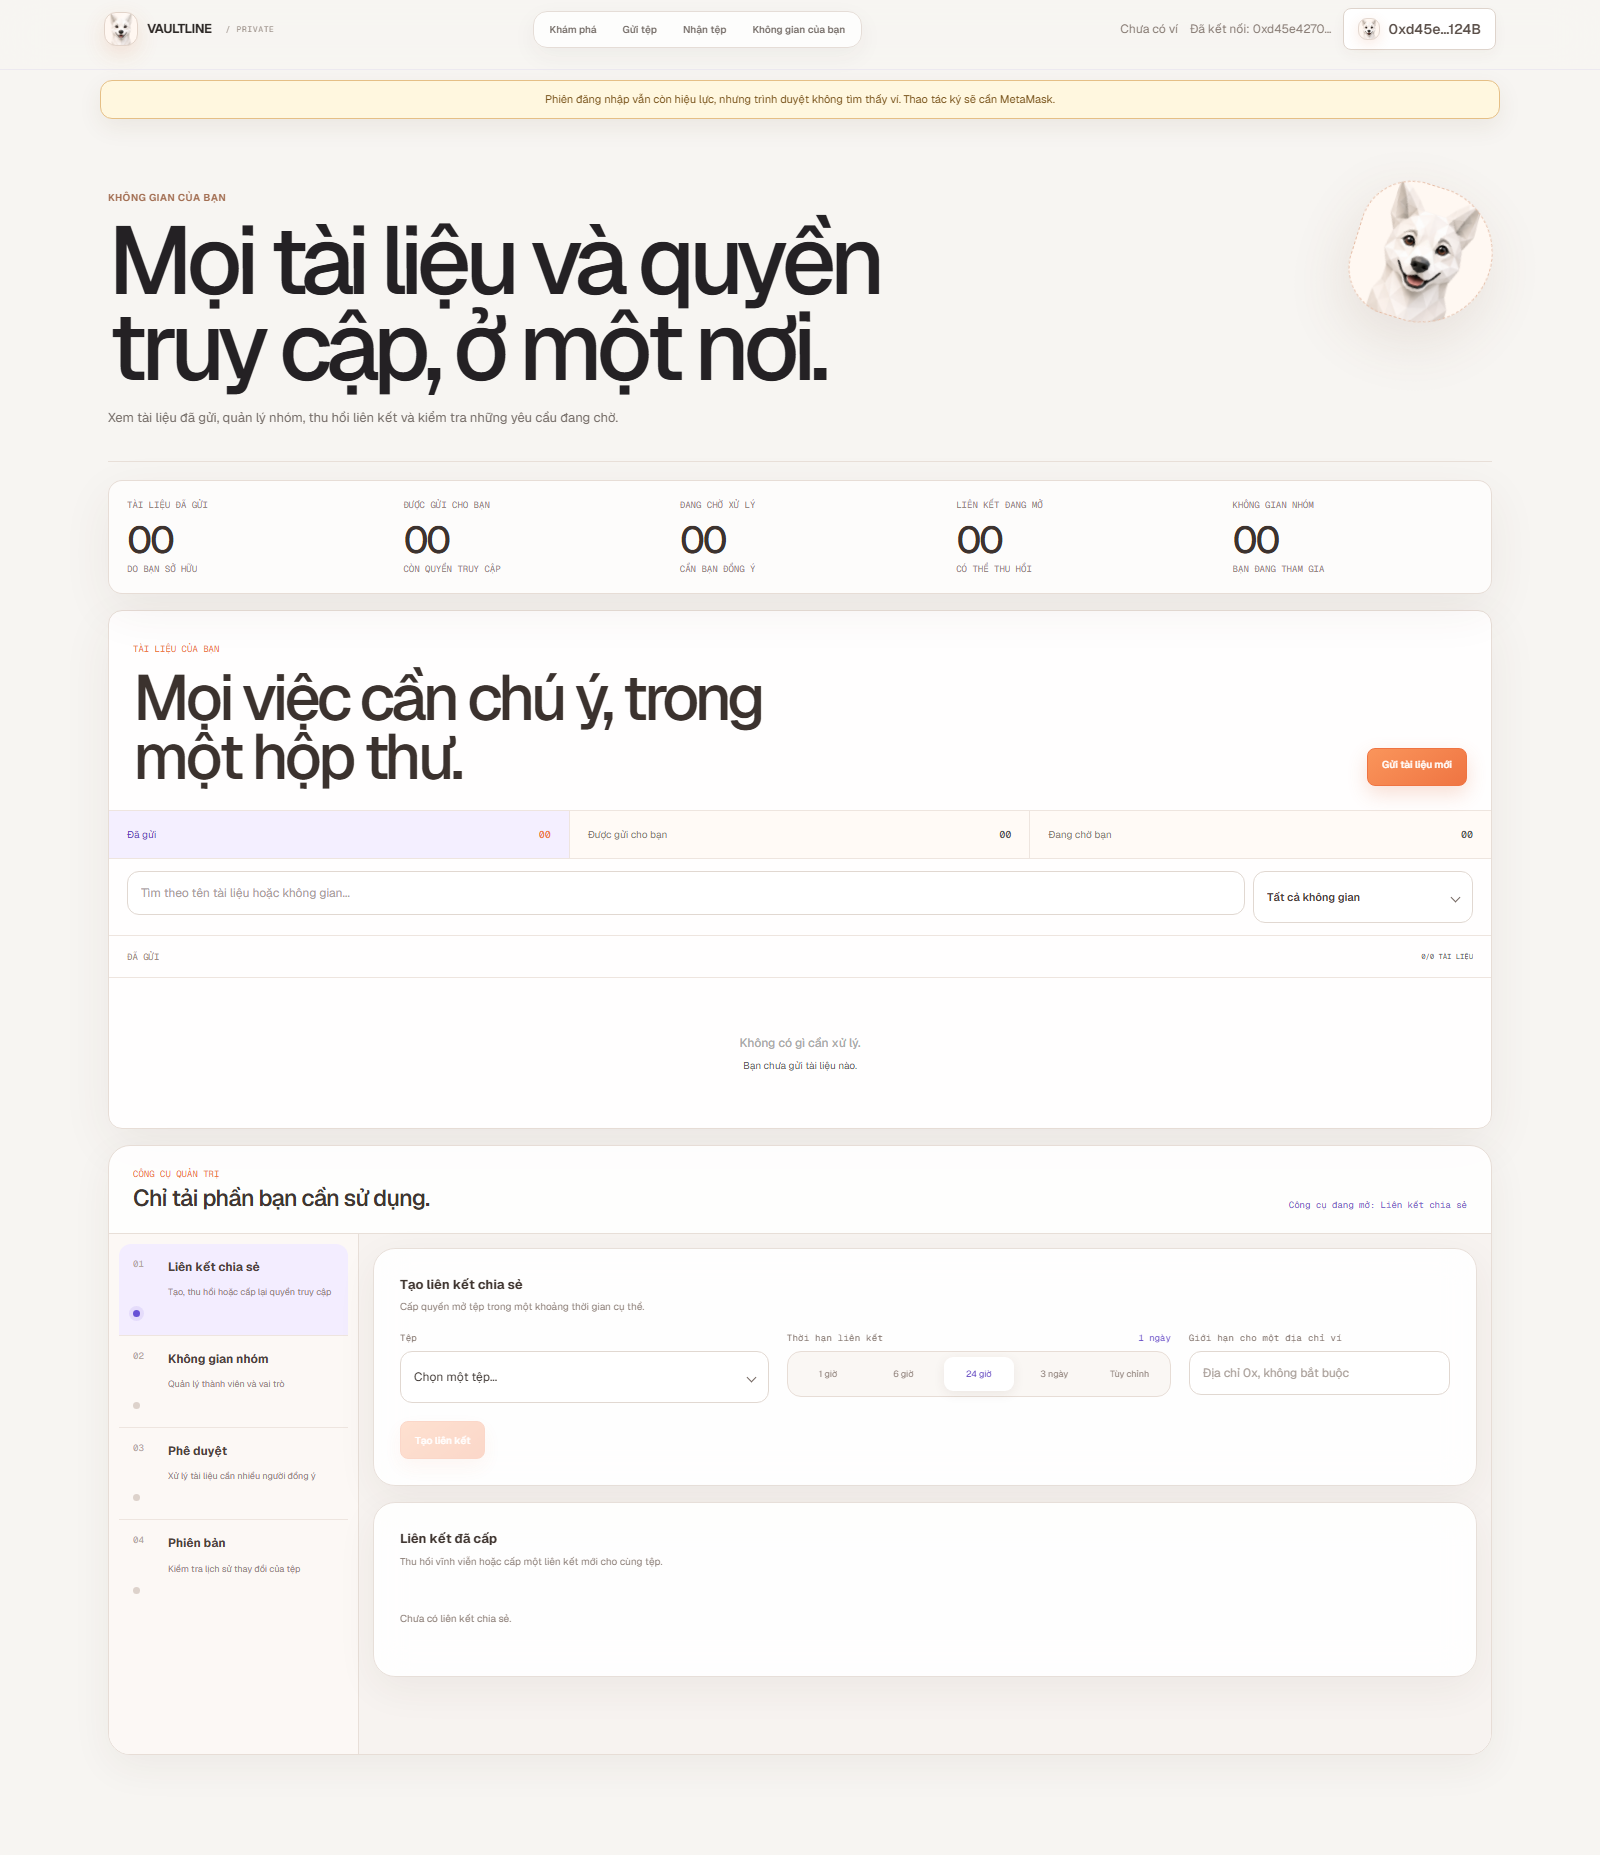
\includegraphics[width=\textwidth,height=0.74\textheight,keepaspectratio]{live-dashboard.png}
\caption{Dashboard quản lý tài liệu, kho và yêu cầu}
\end{figure}

\begin{figure}[H]
\centering
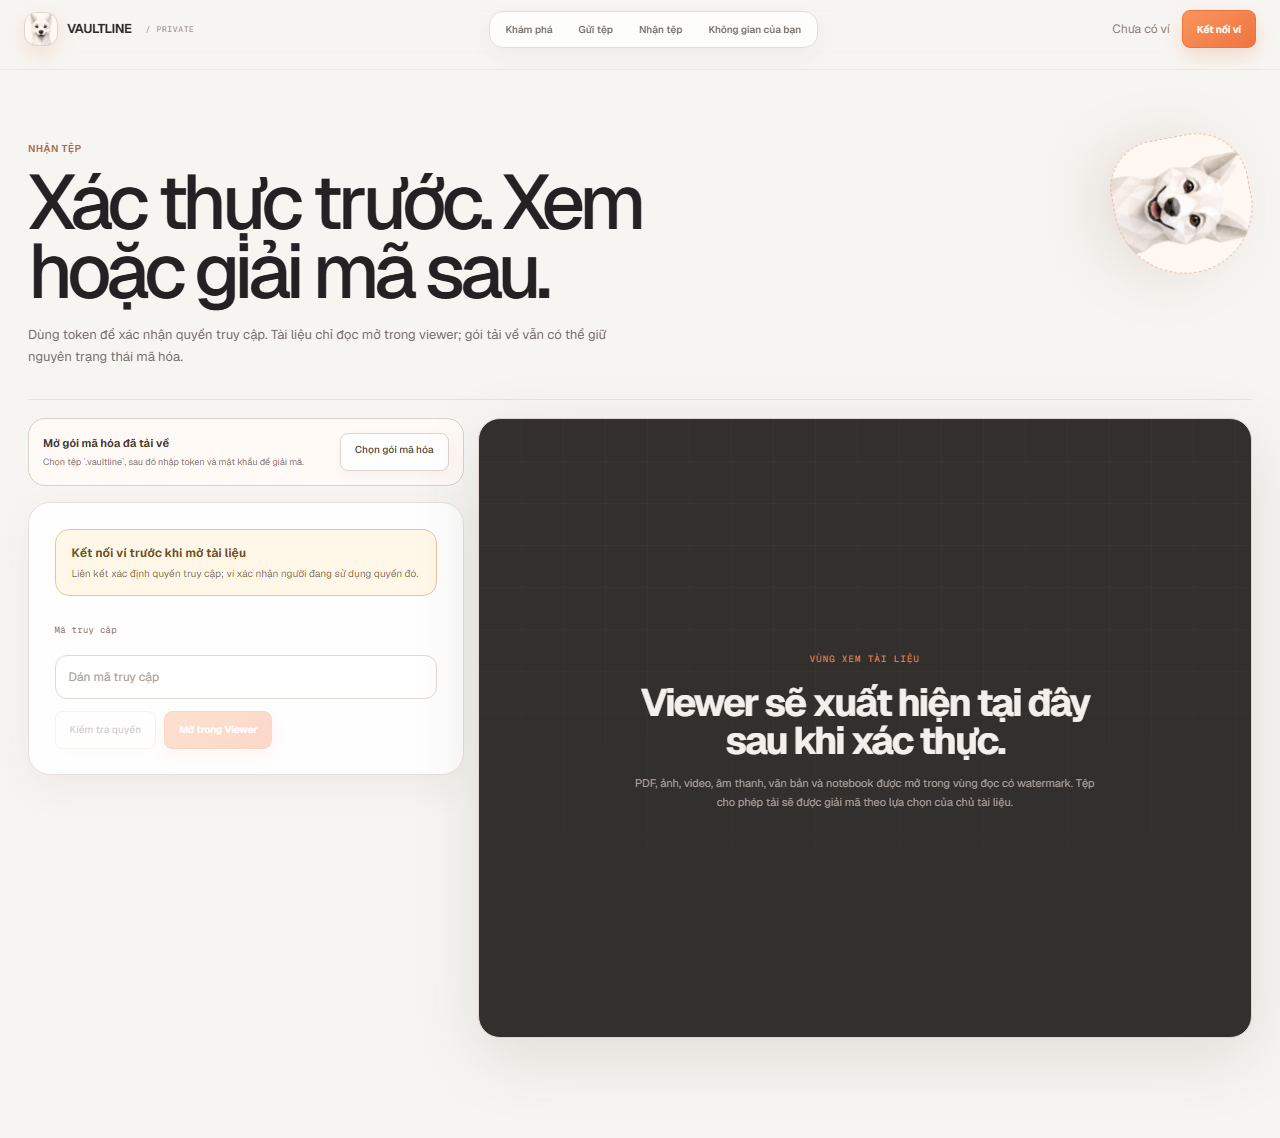
\includegraphics[width=\textwidth,height=0.74\textheight,keepaspectratio]{live-download.png}
\caption{Luồng nhận tài liệu và protected viewer}
\end{figure}

\clearpage

\chapter*{CHƯƠNG 4: CÀI ĐẶT HỆ THỐNG}
\addcontentsline{toc}{chapter}{CHƯƠNG 4: CÀI ĐẶT HỆ THỐNG}

Chương này mô tả cách các thiết kế ở chương trước được hiện thực trong mã nguồn. Nội dung tập trung vào các module quan trọng: xác thực ví, mã hóa, storage, token, approval, dashboard và triển khai.

\section*{4.1. Môi trường và công nghệ}
\addcontentsline{toc}{section}{4.1. Môi trường và công nghệ}

\begin{table}[H]
\centering
\caption{Môi trường cài đặt}
\begin{tabularx}{\textwidth}{|p{4cm}|X|}
\hline
\textbf{Thành phần} & \textbf{Công nghệ} \\ \hline
Frontend & Next.js 15, React 19, TypeScript \\ \hline
Styling/UI & CSS module/global CSS, component tự xây dựng \\ \hline
Wallet & MetaMask, Ethers.js \\ \hline
Mã hóa & Web Crypto API, AES-GCM, ECDH/PBKDF2 theo luồng tương ứng \\ \hline
Backend & Next.js API Routes chạy Node.js runtime \\ \hline
Database & SQLite với better-sqlite3 \\ \hline
Storage & Local filesystem hoặc Cloudflare R2 qua AWS S3 SDK \\ \hline
Deploy & Dockerfile, Railway, persistent volume \\ \hline
Kiểm thử & ESLint, Next build, Playwright \\ \hline
\end{tabularx}
\end{table}

\section*{4.2. Cài đặt xác thực ví}
\addcontentsline{toc}{section}{4.2. Cài đặt xác thực ví}

Xác thực ví được tách thành hai endpoint. Endpoint \code{/api/auth/start} sinh thông điệp cần ký. Endpoint \code{/api/auth/verify} nhận địa chỉ ví và chữ ký, sau đó dùng thư viện \code{ethers} để khôi phục địa chỉ ký. Nếu địa chỉ khôi phục trùng với địa chỉ gửi lên, server tạo session JWT và lưu trong cookie.

Cách cài đặt này giúp hệ thống:

\begin{itemize}
  \item Không cần lưu mật khẩu.
  \item Ràng buộc hành động với địa chỉ ví.
  \item Dễ mở rộng sang các chính sách phân quyền theo ví.
\end{itemize}

\section*{4.3. Cài đặt lưu trữ metadata}
\addcontentsline{toc}{section}{4.3. Cài đặt lưu trữ metadata}

Module \code{src/lib/db.ts} chịu trách nhiệm mở SQLite database và chạy migration. Đường dẫn database lấy từ biến môi trường \code{DB\_PATH}. Khi chạy local, đường dẫn thường là \code{data/app.sqlite}. Khi chạy Railway, đường dẫn là \code{/app/data/app.sqlite} để dữ liệu nằm trong volume.

Migration được viết trực tiếp trong code để prototype dễ chạy. Khi database chưa có bảng, hệ thống tự tạo bảng. Khi phát triển thêm trường mới, code kiểm tra \code{PRAGMA table\_info} và thêm cột còn thiếu. Cách này phù hợp với phạm vi môn học vì giảm bước cấu hình thủ công.

\section*{4.4. Cài đặt storage provider}
\addcontentsline{toc}{section}{4.4. Cài đặt storage provider}

Module \code{src/lib/storage.ts} cung cấp cùng một interface cho hai provider:

\begin{itemize}
  \item \code{local}: ghi ciphertext vào thư mục \code{storage/}.
  \item \code{r2}: ghi ciphertext vào Cloudflare R2 bằng S3-compatible API.
\end{itemize}

Provider được chọn bằng biến môi trường \code{STORAGE\_PROVIDER}. Khi dùng R2, hệ thống yêu cầu account ID, bucket, access key ID và secret access key tương ứng. Các giá trị bí mật chỉ được đặt trong biến môi trường.

Để tránh trùng object, cid được tạo bằng SHA-256 trên ciphertext. Vì cid sinh từ ciphertext, cùng một ciphertext sẽ cho cùng cid.

\section*{4.5. Cài đặt upload và metadata file}
\addcontentsline{toc}{section}{4.5. Cài đặt upload và metadata file}

Khi client gửi metadata tới \code{/api/files}, backend kiểm tra:

\begin{itemize}
  \item Người dùng đã đăng nhập hay chưa.
  \item CSRF token có hợp lệ không.
  \item Các trường bắt buộc như \code{cid}, \code{iv}.
  \item Kích thước file có vượt giới hạn không.
  \item Key material thuộc đúng một chế độ: wrapped key, recipient envelope hoặc threshold shares.
  \item Nếu file thuộc vault, người dùng có quyền ghi hay không.
\end{itemize}

Sau khi hợp lệ, hệ thống lưu bản ghi vào bảng files, tạo token, lưu share nếu có và ghi audit event.

\section*{4.6. Cài đặt phê duyệt ngưỡng}
\addcontentsline{toc}{section}{4.6. Cài đặt phê duyệt ngưỡng}

Phê duyệt ngưỡng được hiện thực bằng nhóm bảng threshold file, threshold share, approval request và approval contribution. Khi người nhận tạo yêu cầu, hệ thống lưu trạng thái \code{pending}. Khi người duyệt gửi approval, API kiểm tra tư cách thành viên và lưu contribution.

Khi số contribution hợp lệ đạt ngưỡng, hệ thống:

\begin{enumerate}
  \item Cập nhật yêu cầu sang trạng thái \code{approved}.
  \item Tạo token mục đích \code{approval}.
  \item Gắn token với requester.
  \item Cho phép requester dùng token để lấy ciphertext và contribution cần thiết.
\end{enumerate}

\section*{4.7. Cài đặt dashboard và protected viewer}
\addcontentsline{toc}{section}{4.7. Cài đặt dashboard và protected viewer}

Dashboard tập hợp nhiều chức năng vào một workspace: tài liệu đã gửi, tài liệu nhận, kho nhóm, yêu cầu phê duyệt, token và phiên bản. Các component được tách theo từng nhóm chức năng để giảm phụ thuộc và thuận tiện bảo trì.

Protected viewer nằm trong luồng download. Viewer chỉ hiển thị nội dung sau khi token hợp lệ và client giải mã thành công. Với một số loại file như ảnh, video hoặc notebook, viewer có thể hiển thị theo kiểu tương ứng; với loại chưa hỗ trợ, hệ thống vẫn có thể cung cấp trạng thái rõ ràng cho người dùng.

\section*{4.8. Cài đặt triển khai}
\addcontentsline{toc}{section}{4.8. Cài đặt triển khai}

Repository có \code{Dockerfile} và \code{railway.json}. Dockerfile build Next.js ở chế độ standalone. Railway dùng healthcheck \code{/api/health}. SQLite được cấu hình tại \code{/app/data/app.sqlite}. Cloudflare R2 được cấu hình qua biến môi trường.

Một lỗi thực tế khi triển khai là quyền ghi vào Railway volume. Vì Railway mount volume ở runtime, container cần đảm bảo tiến trình có quyền ghi vào \code{/app/data}. Dự án đã điều chỉnh Dockerfile để tránh lỗi SQLite không ghi được vào volume trong demo.

\clearpage

\chapter*{CHƯƠNG 5: KIỂM THỬ, TRIỂN KHAI VÀ ĐÁNH GIÁ}
\addcontentsline{toc}{chapter}{CHƯƠNG 5: KIỂM THỬ, TRIỂN KHAI VÀ ĐÁNH GIÁ}

Chương này trình bày chiến lược kiểm thử, kết quả kiểm tra, phương án triển khai và đánh giá hệ thống sau khi cài đặt.

\section*{5.1. Chiến lược kiểm thử}
\addcontentsline{toc}{section}{5.1. Chiến lược kiểm thử}

Hệ thống được kiểm thử theo nhiều tầng:

\begin{table}[H]
\centering
\caption{Chiến lược kiểm thử}
\begin{tabularx}{\textwidth}{|p{3.2cm}|p{4.5cm}|X|}
\hline
\textbf{Tầng kiểm thử} & \textbf{Công cụ} & \textbf{Mục tiêu} \\ \hline
Static analysis & ESLint & Phát hiện lỗi cú pháp, lỗi React/TypeScript và quy tắc code. \\ \hline
Production build & Next.js build & Kiểm tra khả năng compile, type check và build production. \\ \hline
API integration & Playwright request & Kiểm tra auth, token, approval, vault, audit và phân quyền. \\ \hline
End-to-end & Playwright Chromium & Kiểm tra các luồng người dùng trên giao diện. \\ \hline
Runtime healthcheck & \texttt{/api/health} & Kiểm tra database và storage provider khi chạy thật. \\ \hline
\end{tabularx}
\end{table}

\section*{5.2. Ma trận kiểm thử chức năng}
\addcontentsline{toc}{section}{5.2. Ma trận kiểm thử chức năng}

\begin{longtable}{|p{2cm}|p{5.4cm}|p{5.8cm}|}
\caption{Một số test case chính} \\
\hline
\textbf{Mã} & \textbf{Kịch bản} & \textbf{Kỳ vọng} \\ \hline
TC-01 & Truy cập các trang public & Không có lỗi hydration React. \\ \hline
TC-02 & Mở download khi chưa đăng nhập & Nút kiểm tra và mở tài liệu bị vô hiệu hóa. \\ \hline
TC-03 & Gọi healthcheck & API trả về database ready và storage provider. \\ \hline
TC-04 & Đăng ký encryption identity & Public key ký bởi đúng ví được lưu; chữ ký ví khác bị từ chối. \\ \hline
TC-05 & Tạo token và validate token & Token hợp lệ được chấp nhận; token thu hồi/hết hạn bị từ chối. \\ \hline
TC-06 & Phân quyền vault & Owner/editor/viewer bị giới hạn đúng vai trò. \\ \hline
TC-07 & Phê duyệt ngưỡng & Một approval chưa đủ cấp token; đủ ngưỡng mới cấp token cho requester. \\ \hline
TC-08 & Hủy tài liệu & Chỉ owner được hủy; token liên quan bị thu hồi. \\ \hline
TC-09 & Audit trail & Hành động nhạy cảm sinh audit event và event không thể sửa/xóa. \\ \hline
TC-10 & Nhãn UI & Button/link hiển thị có label để dễ dùng và dễ kiểm thử. \\ \hline
\end{longtable}

\section*{5.3. Kết quả kiểm thử hiện tại}
\addcontentsline{toc}{section}{5.3. Kết quả kiểm thử hiện tại}

Các lệnh kiểm tra thường dùng:

\begin{lstlisting}[language=bash]
npm run lint
npm run build
npm run test:e2e
\end{lstlisting}

Trong quá trình hoàn thiện, nhóm đã chạy lint và build nhiều lần. Production build thành công cho các route chính như trang chủ, upload, download, dashboard và các API route. E2E test bao phủ các luồng như hydration, đăng nhập giả lập bằng ví, kiểm tra token, approval, vault, audit, account menu và quyền truy cập.

\section*{5.4. Triển khai local}
\addcontentsline{toc}{section}{5.4. Triển khai local}

Local là phương án demo dự phòng quan trọng. Khi chạy local, app server chạy trên máy cá nhân nhưng vẫn có thể dùng Cloudflare R2 để lưu ciphertext. Điều này giúp demo được đầy đủ logic cloud storage ngay cả khi Railway gặp sự cố.

Cấu hình local cơ bản:

\begin{lstlisting}
JWT_SECRET=replace-with-a-long-random-secret
REQUIRE_CSRF=true
DB_PATH=data/app.sqlite
STORAGE_PROVIDER=r2
CLOUDFLARE_R2_ACCOUNT_ID=<account_id>
CLOUDFLARE_R2_BUCKET=<bucket_name>
CLOUDFLARE_R2_ACCESS_KEY_ID=<rotated_access_key_id>
CLOUDFLARE_R2_SECRET_ACCESS_KEY=<rotated_secret_access_key>
CLOUDFLARE_R2_KEY_PREFIX=ciphertexts
\end{lstlisting}

Chạy production local:

\begin{lstlisting}[language=bash]
npm run build
npm run start
\end{lstlisting}

\section*{5.5. Triển khai Railway và Cloudflare R2}
\addcontentsline{toc}{section}{5.5. Triển khai Railway và Cloudflare R2}

Triển khai online gồm hai phần: Railway chạy ứng dụng và Cloudflare R2 lưu ciphertext. SQLite được lưu trong Railway volume mount tại \texttt{/app/data}. Các biến môi trường quan trọng gồm \texttt{JWT\_SECRET}, \texttt{DB\_PATH}, \texttt{STORAGE\_PROVIDER} và các R2 access key.

Healthcheck sau khi deploy:

\begin{lstlisting}
https://<domain>.up.railway.app/api/health
\end{lstlisting}

Kết quả mong đợi:

\begin{lstlisting}
{
  "ok": true,
  "database": "ready",
  "storageProvider": "r2"
}
\end{lstlisting}

\section*{5.6. Đánh giá hệ thống}
\addcontentsline{toc}{section}{5.6. Đánh giá hệ thống}

\subsection*{5.6.1. Kết quả đạt được}
\addcontentsline{toc}{subsection}{5.6.1. Kết quả đạt được}

Hệ thống đã đạt các mục tiêu chính:

\begin{itemize}
  \item Có prototype web hoạt động với giao diện dashboard, upload và viewer.
  \item Có đăng nhập bằng MetaMask.
  \item Có mã hóa phía client và lưu ciphertext.
  \item Có token truy cập, thu hồi token và hủy tài liệu.
  \item Có luồng phê duyệt A+B cho C.
  \item Có audit trail và kiểm thử tự động.
  \item Có cấu hình local/R2/Railway phục vụ demo.
\end{itemize}

\subsection*{5.6.2. Hạn chế}
\addcontentsline{toc}{subsection}{5.6.2. Hạn chế}

Một số hạn chế cần nêu rõ:

\begin{itemize}
  \item Protected viewer không thể ngăn người dùng chụp ảnh bằng thiết bị khác.
  \item SQLite phù hợp prototype một instance, chưa phù hợp scale nhiều instance.
  \item Chưa có hệ thống notification để báo người duyệt khi có yêu cầu mới.
  \item Chưa có watermark cá nhân hóa theo người nhận.
  \item Chưa có audit receipt dạng Merkle tree hoặc bằng chứng zero-knowledge.
\end{itemize}

\clearpage

\chapter*{CHƯƠNG 6: KẾT LUẬN VÀ HƯỚNG PHÁT TRIỂN}
\phantomsection
\addcontentsline{toc}{chapter}{CHƯƠNG 6: KẾT LUẬN VÀ HƯỚNG PHÁT TRIỂN}

\section*{6.1. Kết luận}
\phantomsection
\addcontentsline{toc}{section}{6.1. Kết luận}

Báo cáo đã trình bày quá trình xây dựng \projectname{} theo góc nhìn Kỹ thuật phần mềm. Từ bài toán chia sẻ tài liệu nhạy cảm, nhóm đã phân tích yêu cầu, xác định tác nhân, thiết kế use case, thiết kế kiến trúc, cơ sở dữ liệu, API, giao diện, sau đó cài đặt và kiểm thử prototype.

Kết quả quan trọng nhất của đề tài là chứng minh được một luồng bảo vệ tài liệu có tính hệ thống: tài liệu được mã hóa trước khi upload, quyền truy cập được cấp bằng token, tài liệu nhạy cảm có thể yêu cầu nhiều người phê duyệt, và chủ sở hữu có thể thu hồi token hoặc hủy tài liệu. Hệ thống cũng có dashboard, viewer, audit trail và cấu hình triển khai lên Railway/R2.

Đối với môn Kỹ thuật phần mềm, đề tài thể hiện đầy đủ các khía cạnh của một quy trình phát triển phần mềm: yêu cầu, thiết kế, cài đặt, kiểm thử, triển khai và đánh giá. Đây không chỉ là một chức năng mã hóa/giải mã, mà là một prototype có nhiều module phối hợp với nhau.

\section*{6.2. Bài học rút ra}
\phantomsection
\addcontentsline{toc}{section}{6.2. Bài học rút ra}

Trong quá trình thực hiện, nhóm rút ra một số bài học:

\begin{itemize}
  \item Cần phân biệt rõ giữa bảo mật bằng mã hóa và kiểm soát hành vi sau khi người dùng đã xem tài liệu.
  \item Thiết kế module rõ ràng giúp hệ thống dễ mở rộng từ local storage sang R2.
  \item Kiểm thử E2E rất cần thiết vì nhiều lỗi chỉ xuất hiện khi các module UI, API, database và session chạy cùng nhau.
  \item Deploy online không chỉ là đẩy code, mà còn phụ thuộc biến môi trường, secret, volume, healthcheck và quyền ghi runtime.
  \item Với hệ thống liên quan quyền truy cập, audit log và thông báo lỗi rõ ràng quan trọng không kém chức năng chính.
\end{itemize}

\section*{6.3. Hướng phát triển}
\phantomsection
\addcontentsline{toc}{section}{6.3. Hướng phát triển}

Các hướng phát triển ngắn hạn:

\begin{itemize}
  \item Thêm watermark cá nhân hóa trong protected viewer để giảm rủi ro chia sẻ trái phép.
  \item Hỗ trợ viewer tốt hơn cho PDF, notebook, video và file khoa học.
  \item Thêm notification khi có yêu cầu phê duyệt mới hoặc file sắp hết hạn.
  \item Cải thiện dashboard audit để chủ sở hữu dễ hiểu hành vi truy cập.
  \item Chuyển SQLite sang PostgreSQL nếu cần nhiều instance hoặc nhiều người dùng.
\end{itemize}

Các hướng nghiên cứu nâng cao:

\begin{itemize}
  \item \textbf{Merkle audit receipt}: tạo biên nhận audit bất biến sau mỗi phiên chia sẻ.
  \item \textbf{Zero-knowledge permission proof}: chứng minh người dùng có quyền mà server không cần biết toàn bộ thông tin định danh.
  \item \textbf{Time-locked encryption}: khóa chỉ có thể giải mã trong khoảng thời gian nhất định.
  \item \textbf{Risk scoring}: đánh giá rủi ro theo thiết bị, tần suất mở file và hành vi bất thường.
\end{itemize}

\section*{6.4. Luận điểm bảo vệ}
\phantomsection
\addcontentsline{toc}{section}{6.4. Luận điểm bảo vệ}

Khi bảo vệ, nhóm cần nhấn mạnh rằng hệ thống không tuyên bố làm cho việc copy trở nên bất khả thi. Nếu người dùng đã được xem nội dung, vẫn tồn tại rủi ro chụp màn hình hoặc copy thủ công. Giá trị của hệ thống nằm ở việc làm cho quyền truy cập trở nên có chủ đích, có thể thu hồi, có thể kiểm chứng và khó bị lạm dụng hơn so với gửi file gốc trực tiếp.

\clearpage

\chapter*{TÀI LIỆU THAM KHẢO}
\phantomsection
\addcontentsline{toc}{chapter}{TÀI LIỆU THAM KHẢO}

\begin{enumerate}
  \item Nhóm 11, \textit{Mã nguồn hệ thống WEB3demo}, GitHub repository. Truy cập ngày 16/06/2026 tại \url{https://github.com/Poicitaco/WEB3demo}.
  \item Vercel, \textit{Next.js Documentation: App Router and Route Handlers}. Truy cập ngày 16/06/2026 tại \url{https://nextjs.org/docs}.
  \item Meta Platforms, \textit{React Reference}. Truy cập ngày 16/06/2026 tại \url{https://react.dev/reference/react}.
  \item Mozilla Developer Network, \textit{Web Crypto API}. Truy cập ngày 16/06/2026 tại \url{https://developer.mozilla.org/en-US/docs/Web/API/Web_Crypto_API}.
  \item MetaMask, \textit{MetaMask Developer Documentation}. Truy cập ngày 16/06/2026 tại \url{https://docs.metamask.io}.
  \item Ethers.js, \textit{Ethers Documentation, Signing Messages}. Truy cập ngày 16/06/2026 tại \url{https://docs.ethers.org/v6}.
  \item Cloudflare, \textit{Cloudflare R2 Object Storage Documentation}. Truy cập ngày 16/06/2026 tại \url{https://developers.cloudflare.com/r2}.
  \item Railway, \textit{Railway Documentation: Deployments and Volumes}. Truy cập ngày 16/06/2026 tại \url{https://docs.railway.com}.
  \item SQLite Consortium, \textit{SQLite Documentation}. Truy cập ngày 16/06/2026 tại \url{https://www.sqlite.org/docs.html}.
  \item Microsoft, \textit{Playwright Documentation}. Truy cập ngày 16/06/2026 tại \url{https://playwright.dev/docs/intro}.
  \item OWASP Foundation, \textit{Web Security Testing Guide}. Truy cập ngày 16/06/2026 tại \url{https://owasp.org/www-project-web-security-testing-guide}.
  \item NIST, \textit{Recommendation for Block Cipher Modes of Operation: Galois/Counter Mode (GCM)}, NIST SP 800-38D, 2007. \url{https://csrc.nist.gov/publications/detail/sp/800-38d/final}.
  \item NIST, \textit{Advanced Encryption Standard (AES)}, FIPS PUB 197, 2023. \url{https://csrc.nist.gov/pubs/fips/197/final}.
\end{enumerate}


\end{document}
